\documentclass[a4paper]{article}
\usepackage[a4paper,left=3cm,right=2.5cm,top=2.5cm,bottom=2.5cm]{geometry}
\usepackage[utf8]{inputenc}
\usepackage{enumerate}
\usepackage{graphicx}
\usepackage{ccicons}
\usepackage{amssymb} % Simbolos matematicos
\usepackage{xcolor}
\usepackage{color}
\usepackage{fancyvrb}
\usepackage{url}
\usepackage{caption}
\usepackage{amsfonts}
\usepackage{amsmath,amscd}
\usepackage{frame}
\usepackage{mdframed}
\usepackage{listings}
\usepackage{wrapfig,lipsum}
\usepackage{imakeidx}
\usepackage{pdfpages}
\usepackage[pdfpagelabels,bookmarks,hyperindex,hyperfigures]{hyperref}
\definecolor{bluelink}{RGB}{0,0,238}
\begin{document}

\lstdefinelanguage{Rips}{%
  keywords={consts, vars, rules,levels,int,string,bool,float},
  keywordstyle=\color{teal}\bfseries,
  ndkeywords={soft, true, false},
  ndkeywordstyle=\color{bluelink}\bfseries,
  identifierstyle=\color{black},
  sensitive=rue,
  comment=[l]{\#},
  commentstyle=\color{gray}\ttfamily,
  stringstyle=\color{red}\ttfamily,
  morestring=[b]"
}


\lstdefinestyle{rips}{ % add your own preferences
    basicstyle=\footnotesize,
    keywordstyle=\color{red},
    numbers=left,
    numbersep=10pt,
    showstringspaces=false,
    stringstyle=\color{blue},
    tabsize=4,
    language=Rips
}
\lstset{language=Rips, style=rips}

\title{Technical report: Implementation of the Robotic Intrusion
Prevention System (RIPS) research prototype}
\author{Gorka Guardiola Múzquiz, Enrique Soriano-Salvador\\
\centering \footnotesize GSyC, Universidad Rey Juan Carlos}
\date{\today}

\maketitle
\section{Introduction}
We introduced the need for a Robotic Intrusion Prevention System (RIPS
from now on) in~\cite{rips}. This document describes the implementation
of a complete RIPS research prototype.

The prototype is divided in two main components:

\begin{itemize}
	\item A monitor used to capture the interactions of ROS 2 nodes
	following the Publisher/Subscriber model which reacts to changes
	in the computation graph (i.e. the set of participants, topics,
	available in the system).

	The monitor is a regular ROS 2
	participant subscribed to all the topics in the ROS system
	(i.e. domain).

	\item A RIPS engine that defines and evaluates the rules to trigger different
	mitigation actions. In~\cite{rips} we delineated the requisites and a
	rough design for a DSL (Domain Specific Language) to specify rules for
	the RIPS.

	These rules will be evaluated for each monitored message, triggering
	actions if something untoward is detected. In
	this document we present a concrete implementation of the RIPS and the
	design decisions we have taken while creating it.
\end{itemize}

In the next section we explain the architecture of the system.

\section{Architecture and Requisites}

Figure~\ref{fig:arch} shows the architecture of the prototype.
The elements in the figure are:

\begin{itemize}
	\item The robot's components interact by means of the ROS 2 communication mechanisms
	based on the Publisher/Subscriber model.

	\item RIPS is an additional
	ROS 2 participant in the robotic system. It is subscribed to all the topics
	in the robotic system. It also detects all the participants, available
	topics, etc. in the system. As stated before, RIPS is formed by
	two main components (the monitor and the engine).
	The implementation of these components is described in the following sections.

	\item RIPS is focused on mitigation at the robotic level. In this implementation, RIPS uses
	\textit{System Modes}~\cite{9474424} to change the behavior of the
	robot's components in case of intrusion.

	RIPS maintains a thread level indicator, that can be mapped (one to one) to different
	System Modes. When the RIPS alert level changes, RIPS notifies the System
	Modes mechanisms to alter the state of the rest of nodes.

	\item Nevertheless, RIPS is able to execute external commands and create alarms
	for a conventional IDS/IPS actions (e.g. Snort). Standard IPS mechanisms
	should be activated through commands (e.g. applying firewall configurations).

	\item External programs (and the admin, or operator) are able to
	send events to RIPS. This is done through UNIX signals. The engine
	can catch and recognize such events, so they can be used by the
	user-defined rules (the \texttt{rules.rul} file in the Figure).
\end{itemize}

\begin{figure}[t!]
\begin{center}
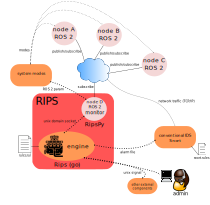
\includegraphics[width=\textwidth]{figs/svg_arch.pdf}
\caption{RIPS architecture \label{fig:arch}}
\end{center}
\end{figure}


RIPS is a detection system that operates at the robotic system's level.
Therefore, the RIPS program is a regular ROS 2 participant.
ROS 2 is a robotic framework built over a DDS (Data Distribution Service)
middleware implementation, specifically over the RTPS
(Real Time Publish Subscribe) protocol specification~\cite{rtps-doc}.
There are multiple DDS vendors that can be used by
ROS 2.

RIPS stipulates two prerequisites for the ROS 2 system configuration:

\begin{enumerate}
	\item \textbf{The ROS 2 security mechanisms for authentication, confidentiality,
	integrity,
	and access control must be correctly configured and enabled}
	(i.e., the environment variable
       \texttt{ROS\_SECURITY\_ENABLE} must be set to \texttt{true}).
	ROS 2 security must be set to \textit{strict mode} (i.e., the \texttt{ROS\_SECURITY\_STRATEGY}
	must be set to \texttt{Enforce}). In this mode, if the configuration files
	for security are missing or incorrect, the ROS2 node cannot be executed.

	The ROS 2 nodes must use correct \emph{keystores}: Each node only has its own private key
	and the public keys and certificates needed to communicate with the other components.
	The private key of the root certificate (CA) used to sign the rest of certificates
	must not be stored in any component of the system.

	\textbf{Rationale:} RIPS rules rely on the identity of the ROS 2
	components of the robotic system. They also rely on the data
	published by those components.
	Thus, unauthorized nodes must not be part of the robotic system.
	Without confidentiality and integrity mechanisms, fake messages could be forged
	and legitimage messages could be modified or removed.

	Note that authenticated nodes can be compromised by attackers. RIPS rules can
	be defined to detect anomalous and malicious behaviors.


	\item \textbf{The transport layer used by the DDS middleware must take
	advantage of the multicast capabilities}.
	For example, for the FastDDS vendor~\cite{fastdds-doc}, the multicast
	capabilities for UDP can be configured in the profile
	XML file of the nodes by defining \textit{multicast locators} like this:

{ \scriptsize
\begin{verbatim}
<!-- enabling multicast for data (topics)-->
<multicastLocatorList>
   <locator>
      <udpv4>
         <address>239.255.0.4</address>
         <port>7900</port>
      </udpv4>
   </locator>
</multicastLocatorList>
</subscriber>


<!-- enabling multicast for data (topics)-->
<publisher profile_name="publisher_xml_conf_multicast_locators_profile">
<multicastLocatorList>
   <locator>
      <udpv4>
         <address>239.255.0.4</address>
         <port>7900</port>
      </udpv4>
   </locator>
</multicastLocatorList>
</publisher>
\end{verbatim}
}

	\textbf{Rationale:} The multicast capabilities are mandatory when using RIPS
	in order to prevent malicious nodes (e.g. hijacked authenticated nodes that were
	properly authenticated) bypassing the ROS 2 monitor. If the robotic system
	relies on unicast communications to send the published messages on a topic
	to the corresponding
	subscribers, malicious publishers can send some messages to
	selected nodes, ignoring the rest of subscribers (e.g. the RIPS monitor).
	This trivial attack would bypass the RIPS detection in the robotic system.

	This prerequisite of making all the communications multicast, forces the publisher to
	send only one message through the wire. This message will be necessarily received
	by all the interested nodes (i.e. all the subscribers for the corresponding topic).
	This way, if a message published on a topic, it will be available for all the
	participants, including the RIPS.

	Moreover, taking advantage of the multicast capabilities
	improves the performance
	of RTPS applications with multiple publishers for a topic~\cite{rtps-doc}:

	\begin{quote}
		If available, RTPS can also take advantage of the multicast
		capabilities of the transport mechanism, where one message from
		a sender can reach multiple receivers.
	\end{quote}
\end{enumerate}

\textbf{Executing RIPS without satisfying these two prerequisites
is feasible; however, it is devoid of purpose or meaningful outcome.}
Henceforth, we suppose the fulfillment of these two prerequisites.


\section{Monitor: RipsPy}

The monitor is implemented by a Python 3 program named \texttt{ripspy.py},
which implements a ROS 2 program.
This program executes the engine on a different process.

The monitor and the engine are connected by a UNIX domain socket. This
inter-process communication (IPC) mechanism is a full-duplex channel.
Bothe the monitor and the engine send events to each others through this socket. The events are
encoded in YAML.

\subsection{Implementation}

The program implements a ROS 2 node class
named \texttt{Ripspy} (derived from the ROS 2 \texttt{Node}
class).

This monitor has two threads:

\begin{enumerate}
	\item The thread used to execute the \texttt{Node}'s main loop.
	This execution flow is used to receive data
	from topics and inspect the computation graph.
	This execution flow executes:

	\begin{itemize}
		\item The reception callback to process the messages
		published in the different topics.

		\item A timer callback, used to execute two
		scheduled tasks:

		\begin{itemize}
			\item Updating the current state of the computation
			graph (from now on, the \textit{context}).
			When a new topic is detected, the monitor
			becomes a subscriber.

			Note that there are some blacklisted topics.
			These topics are ignored by the monitor. For example,
			\texttt{/rosout} is always in the black list,
			because it produces feedback loops in the monitor.
			The user can add other
			topics to this black list, by using an environment
			variable (see Section~\ref{sec:env}).

			\item Processing events sent from the engine to
			the monitor, which
			are stored in a thread-safe queue structure.
			Those events are:

			\begin{itemize}
				\item A change of the current RIPS level.

				\item Alerts.
			\end{itemize}
		\end{itemize}
	\end{itemize}

	\item The thread that reads messages from the UNIX domain socket
	and stores them in the thread-safe queue. This thread does not
	use any ROS 2 function. It performs blocking read operations
	on the socket.
\end{enumerate}

These two threads only share the thread-safe queue.
The idea is to isolate all the ROS 2 activity (calls to the \texttt{rclpy}
library functions, handlers, etc.) in one thread, to avoid
race conditions. Figure~\ref{fig:threads} depicts the basic scheme of
this program.

\begin{figure}[t!]
\begin{center}
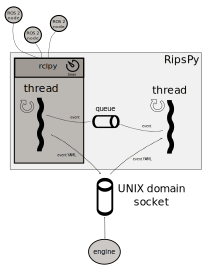
\includegraphics[width=0.7\textwidth]{figs/svg_ripspythreads.pdf}
\caption{RipsPy scheme \label{fig:threads}}
\end{center}
\end{figure}

The monitor sends two different events to the engine through the
socket, serialized in YAML. A new message is sent
from the monitor to the engine when:

\begin{itemize}
	\item The context changes: There are changes in the topics,
	nodes, etc.

	\item A message is received from a topic.
\end{itemize}

The engine reacts to these events, evaluating the corresponding
rules (as will be described in Section~\ref{sect:rips}).

\subsection{Environment \label{sec:env}}

RIPS uses the following environment variables:

\begin{itemize}
	\item \texttt{RIPSRULES}: The path for the rules file used by
		the engine. This variable is mandatory.

	\item \texttt{RIPSSCRIPTS}: The path for the scripts needed by
		the engine. This variable is mandatory.

	\item \texttt{RIPSBLACKLIST}: The list of ignored topics,
	separated by `:'. Note that the topic
	\texttt{/rosout} is always ignored (even when this variable
	is not defined).

	\item \texttt{RIPSSOCKET}: The path for the Unix domain socket
		used to communicate with the engine.
		The default path is \texttt{/tmp/rips.socket}.

	\item \texttt{RIPSTEESOCKET}: The path for the Unix domain socket
		used by \texttt{ripsdash} (see Section \ref{sec:dash}. If
		the variable is defined and \texttt{ripsdash} is not running,
		the program will fail.
\end{itemize}


\subsection{Context}

The monitor executes periodically a method to retrieve de current
ROS 2 context. This is done by calling the following methods:

\begin{itemize}
	\item  The \texttt{get\_node\_names}
	method of the \texttt{Node} class to retrieve the list
	of known nodes.

	\item For each detected node, the \texttt{get\_service\_names\_and\_types\_by\_node}
	method is invoked to retrieve its services and types.

	\item The \texttt{get\_topic\_names\_and\_types} method to
	retrieve all the topics and their types.

	\item For each topic, the \texttt{get\_publishers\_info\_by\_topic} and
	\texttt{get\_subscribers\_info\_by\_topic} methods are invoked to get
	the corresponding publishers/subscribers, IDs, etc.
\end{itemize}

A custom representation of the computation
graph is maintained by a class named \texttt{RipsContext}.
It stores:
\begin{itemize}
	\item The discovered topics, including:
	\begin{itemize}
		\item The name.
		\item The parameters.
		\item The list of subscribers.
		\item The list of publishers.
	\end{itemize}
	\item The discovered nodes, including:
	\begin{itemize}
		\item The name.
		\item The GIDS of the node.
		\item The list of services.
	\end{itemize}
\end{itemize}

Note that the RIPS monitor is a regular ROS 2 node, so it will be also
part of the current context (the name of this node is \texttt{rips}).

When the context changes, the monitor sends an event of type \texttt{graph}
(with the complete context) to the engine.

For example, this event describes a context with two nodes (RIPS and
a node named \texttt{recorder}) and several topics.  It also includes
the current level and other relevant information (that will be described
later):

{\scriptsize
\begin{verbatim}
---
currentlevel: __DEFAULT__
currentgrav: 0.0
lastalert: ''
event: graph
context:
  nodes:
    - node: recorder
      gids:
        - f4.f2.83.53.2d.8d.45.7b.10.20.b5.72.00.00.10.03.00.00.00.00.00.00.00.00
        - f4.f2.83.53.2d.8d.45.7b.10.20.b5.72.00.00.11.04.00.00.00.00.00.00.00.00
        - f4.f2.83.53.2d.8d.45.7b.10.20.b5.72.00.00.03.03.00.00.00.00.00.00.00.00
        - f4.f2.83.53.2d.8d.45.7b.10.20.b5.72.00.00.12.04.00.00.00.00.00.00.00.00
        - f4.f2.83.53.2d.8d.45.7b.10.20.b5.72.00.00.13.04.00.00.00.00.00.00.00.00
      services:
        - service: /recorder/describe_parameters
          params:
            - rcl_interfaces/srv/DescribeParameters
        - service: /recorder/get_parameter_types
          params:
            - rcl_interfaces/srv/GetParameterTypes
        - service: /recorder/get_parameters
          params:
            - rcl_interfaces/srv/GetParameters
        - service: /recorder/list_parameters
          params:
            - rcl_interfaces/srv/ListParameters
        - service: /recorder/set_parameters
          params:
            - rcl_interfaces/srv/SetParameters
        - service: /recorder/set_parameters_atomically
          params:
            - rcl_interfaces/srv/SetParametersAtomically
    - node: rips
      gids:
        - 9a.42.c0.75.93.e2.5f.fc.78.54.49.20.00.00.04.03.00.00.00.00.00.00.00.00
        - 9a.42.c0.75.93.e2.5f.fc.78.54.49.20.00.00.11.04.00.00.00.00.00.00.00.00
        - 9a.42.c0.75.93.e2.5f.fc.78.54.49.20.00.00.03.03.00.00.00.00.00.00.00.00
        - 9a.42.c0.75.93.e2.5f.fc.78.54.49.20.00.00.14.04.00.00.00.00.00.00.00.00
        - 9a.42.c0.75.93.e2.5f.fc.78.54.49.20.00.00.15.04.00.00.00.00.00.00.00.00
      services:
        - service: /rips/describe_parameters
          params:
            - rcl_interfaces/srv/DescribeParameters
        - service: /rips/get_parameter_types
          params:
            - rcl_interfaces/srv/GetParameterTypes
        - service: /rips/get_parameters
          params:
            - rcl_interfaces/srv/GetParameters
        - service: /rips/list_parameters
          params:
            - rcl_interfaces/srv/ListParameters
        - service: /rips/set_parameters
          params:
            - rcl_interfaces/srv/SetParameters
        - service: /rips/set_parameters_atomically
          params:
            - rcl_interfaces/srv/SetParametersAtomically
  topics:
    - topic: /parameter_events
      parameters:
        - rcl_interfaces/msg/ParameterEvent
      publishers:
        - recorder
        - rips
      subscribers:
        - recorder
        - rips
    - topic: /rosout
      parameters:
        - rcl_interfaces/msg/Log
      publishers:
        - recorder
        - rips
      subscribers:
        - ~
    - topic: /videocorridor
      parameters:
        - std_msgs/msg/String
      publishers:
        - ~
      subscribers:
        - recorder
        - rips
    - topic: /videooffice
      parameters:
        - std_msgs/msg/String
      publishers:
        - ~
      subscribers:
        - recorder
        - rips
...
\end{verbatim}
}

The engine is stateless: It does not store the context. Events
are self-contained.

\subsection{Subscribing to new topics}


When the monitor detects a new topic, it becomes a subscriber
if the topic is not in the list of ignored topics.
This is done by creating a nested function to be the handler
for the new topic:

\lstinputlisting[language=Python]{src/func.py}

\subsection{Processing messages}


Each message published in any topic is received by the monitor.
Then, the monitor creates an event of type \texttt{message}
and sends it to the engine.

This kind of event includes
the message data and the complete context.
For example, this is an event that describes a message received
from topic \texttt{videooffice}:

{\scriptsize
\begin{verbatim}
---
currentlevel: __DEFAULT__
currentgrav: 0.0
lastalert: ''
event: message
fromtopic: /videooffice
msg:
  data: 'OFFICE CAMERA: SEQ 0'

rawmsg: |
  AAEAABUAAABPRkZJQ0UgQ0FNRVJBOiBTRVEgMAA=

context:
  nodes:
    - node: officecamera
      gids:
        - d0.73.67.8e.a3.6f.88.c8.fe.c2.0c.90.00.00.10.03.00.00.00.00.00.00.00.00
        - d0.73.67.8e.a3.6f.88.c8.fe.c2.0c.90.00.00.11.04.00.00.00.00.00.00.00.00
        - d0.73.67.8e.a3.6f.88.c8.fe.c2.0c.90.00.00.03.03.00.00.00.00.00.00.00.00
        - d0.73.67.8e.a3.6f.88.c8.fe.c2.0c.90.00.00.12.03.00.00.00.00.00.00.00.00
      services:
        - service: /officecamera/describe_parameters
          params:
            - rcl_interfaces/srv/DescribeParameters
        - service: /officecamera/get_parameter_types
          params:
            - rcl_interfaces/srv/GetParameterTypes
        - service: /officecamera/get_parameters
          params:
            - rcl_interfaces/srv/GetParameters
        - service: /officecamera/list_parameters
          params:
            - rcl_interfaces/srv/ListParameters
        - service: /officecamera/set_parameters
          params:
            - rcl_interfaces/srv/SetParameters
        - service: /officecamera/set_parameters_atomically
          params:
            - rcl_interfaces/srv/SetParametersAtomically
    - node: recorder
      gids:
        - f4.f2.83.53.2d.8d.1f.c5.d0.7a.4a.78.00.00.10.03.00.00.00.00.00.00.00.00
        - f4.f2.83.53.2d.8d.1f.c5.d0.7a.4a.78.00.00.11.04.00.00.00.00.00.00.00.00
        - f4.f2.83.53.2d.8d.1f.c5.d0.7a.4a.78.00.00.03.03.00.00.00.00.00.00.00.00
        - f4.f2.83.53.2d.8d.1f.c5.d0.7a.4a.78.00.00.12.04.00.00.00.00.00.00.00.00
        - f4.f2.83.53.2d.8d.1f.c5.d0.7a.4a.78.00.00.13.04.00.00.00.00.00.00.00.00
      services:
        - service: /recorder/describe_parameters
          params:
            - rcl_interfaces/srv/DescribeParameters
        - service: /recorder/get_parameter_types
          params:
            - rcl_interfaces/srv/GetParameterTypes
        - service: /recorder/get_parameters
          params:
            - rcl_interfaces/srv/GetParameters
        - service: /recorder/list_parameters
          params:
            - rcl_interfaces/srv/ListParameters
        - service: /recorder/set_parameters
          params:
            - rcl_interfaces/srv/SetParameters
        - service: /recorder/set_parameters_atomically
          params:
            - rcl_interfaces/srv/SetParametersAtomically
    - node: rips
      gids:
        - 9a.42.c0.75.93.e2.5f.fc.78.54.49.20.00.00.04.03.00.00.00.00.00.00.00.00
        - 9a.42.c0.75.93.e2.5f.fc.78.54.49.20.00.00.11.04.00.00.00.00.00.00.00.00
        - 9a.42.c0.75.93.e2.5f.fc.78.54.49.20.00.00.03.03.00.00.00.00.00.00.00.00
        - 9a.42.c0.75.93.e2.5f.fc.78.54.49.20.00.00.14.04.00.00.00.00.00.00.00.00
        - 9a.42.c0.75.93.e2.5f.fc.78.54.49.20.00.00.15.04.00.00.00.00.00.00.00.00
      services:
        - service: /rips/describe_parameters
          params:
            - rcl_interfaces/srv/DescribeParameters
        - service: /rips/get_parameter_types
          params:
            - rcl_interfaces/srv/GetParameterTypes
        - service: /rips/get_parameters
          params:
            - rcl_interfaces/srv/GetParameters
        - service: /rips/list_parameters
          params:
            - rcl_interfaces/srv/ListParameters
        - service: /rips/set_parameters
          params:
            - rcl_interfaces/srv/SetParameters
        - service: /rips/set_parameters_atomically
          params:
            - rcl_interfaces/srv/SetParametersAtomically
  topics:
    - topic: /parameter_events
      parameters:
        - rcl_interfaces/msg/ParameterEvent
      publishers:
        - officecamera
        - recorder
        - rips
      subscribers:
        - officecamera
        - recorder
        - rips
    - topic: /rosout
      parameters:
        - rcl_interfaces/msg/Log
      publishers:
        - officecamera
        - recorder
        - rips
      subscribers:
        - ~
    - topic: /videocorridor
      parameters:
        - std_msgs/msg/String
      publishers:
        - ~
      subscribers:
        - recorder
        - rips
    - topic: /videooffice
      parameters:
        - std_msgs/msg/String
      publishers:
        - officecamera
      subscribers:
        - recorder
        - rips
...
\end{verbatim}
}

The YAML event includes the deserialized data of the message and the
raw data (serialized in Base 64).

\subsection{Safety Mechanisms: Signaling System Modes}

When the engine changes the current alert level, it sends
an event to the monitor.

The monitor is in charge of signaling
System Modes to activate the new level. This is done via two
mechanisms:

\begin{itemize}
	\item Changing a ROS 2 parameter.
	\item Invoking a ROS 2 service named \texttt{/safety/change\_mode},
	passing the new level name as an argument.
\end{itemize}

This way, the robot will change its behavior as defined by the modes. For
example, it can some devices or forbid some locations or navigation
routes.

\subsection{Execution}

RipsPy is a ROS 2 package.
It can be launched like this\footnote{This example uses FastRTPS as the DDS vendor}:

\begin{verbatim}
$> . install/setup.bash
$> export RMW_IMPLEMENTATION=rmw_fastrtps_cpp
$> export FASTRTPS_DEFAULT_PROFILES_FILE=profiles.xml
$> export RMW_FASTRTPS_USE_QOS_FROM_XML=1
$> export ROS_SECURITY_KEYSTORE=keystore-rips
$> export ROS_SECURITY_ENABLE=true
$> export ROS_SECURITY_STRATEGY=Enforce
$> export RIPSRULES=/tmp/example/r5.rul
$> export RIPSSCRIPTS=/tmp/example/scripts
$> export RIPSTEESOCKET=/tmp/ripstee.socket
$> ros2 run ripspy ripspy --ros-args -e /rips
\end{verbatim}

Note that the last command executes both the monitor and
the engine in separate processes.

\subsection{Visualization \label{sec:dash}}

We have implemented a simple command to visualize inside a terminal (i.e. a TUI
or text-based user interface)
the data transmitted from the monitor to the engine: \texttt{ripsdash.py}.
Figure~\ref{fig:dash} shows an example of the TUI
of this application running.

This program receives
the same YAML data than the engine
and represents the data in the terminal
(topics, nodes and messages) and the current alert level.
An extra Unix socket domain is used to receive the YAML from the monitor.


\begin{figure}[t]
\begin{center}
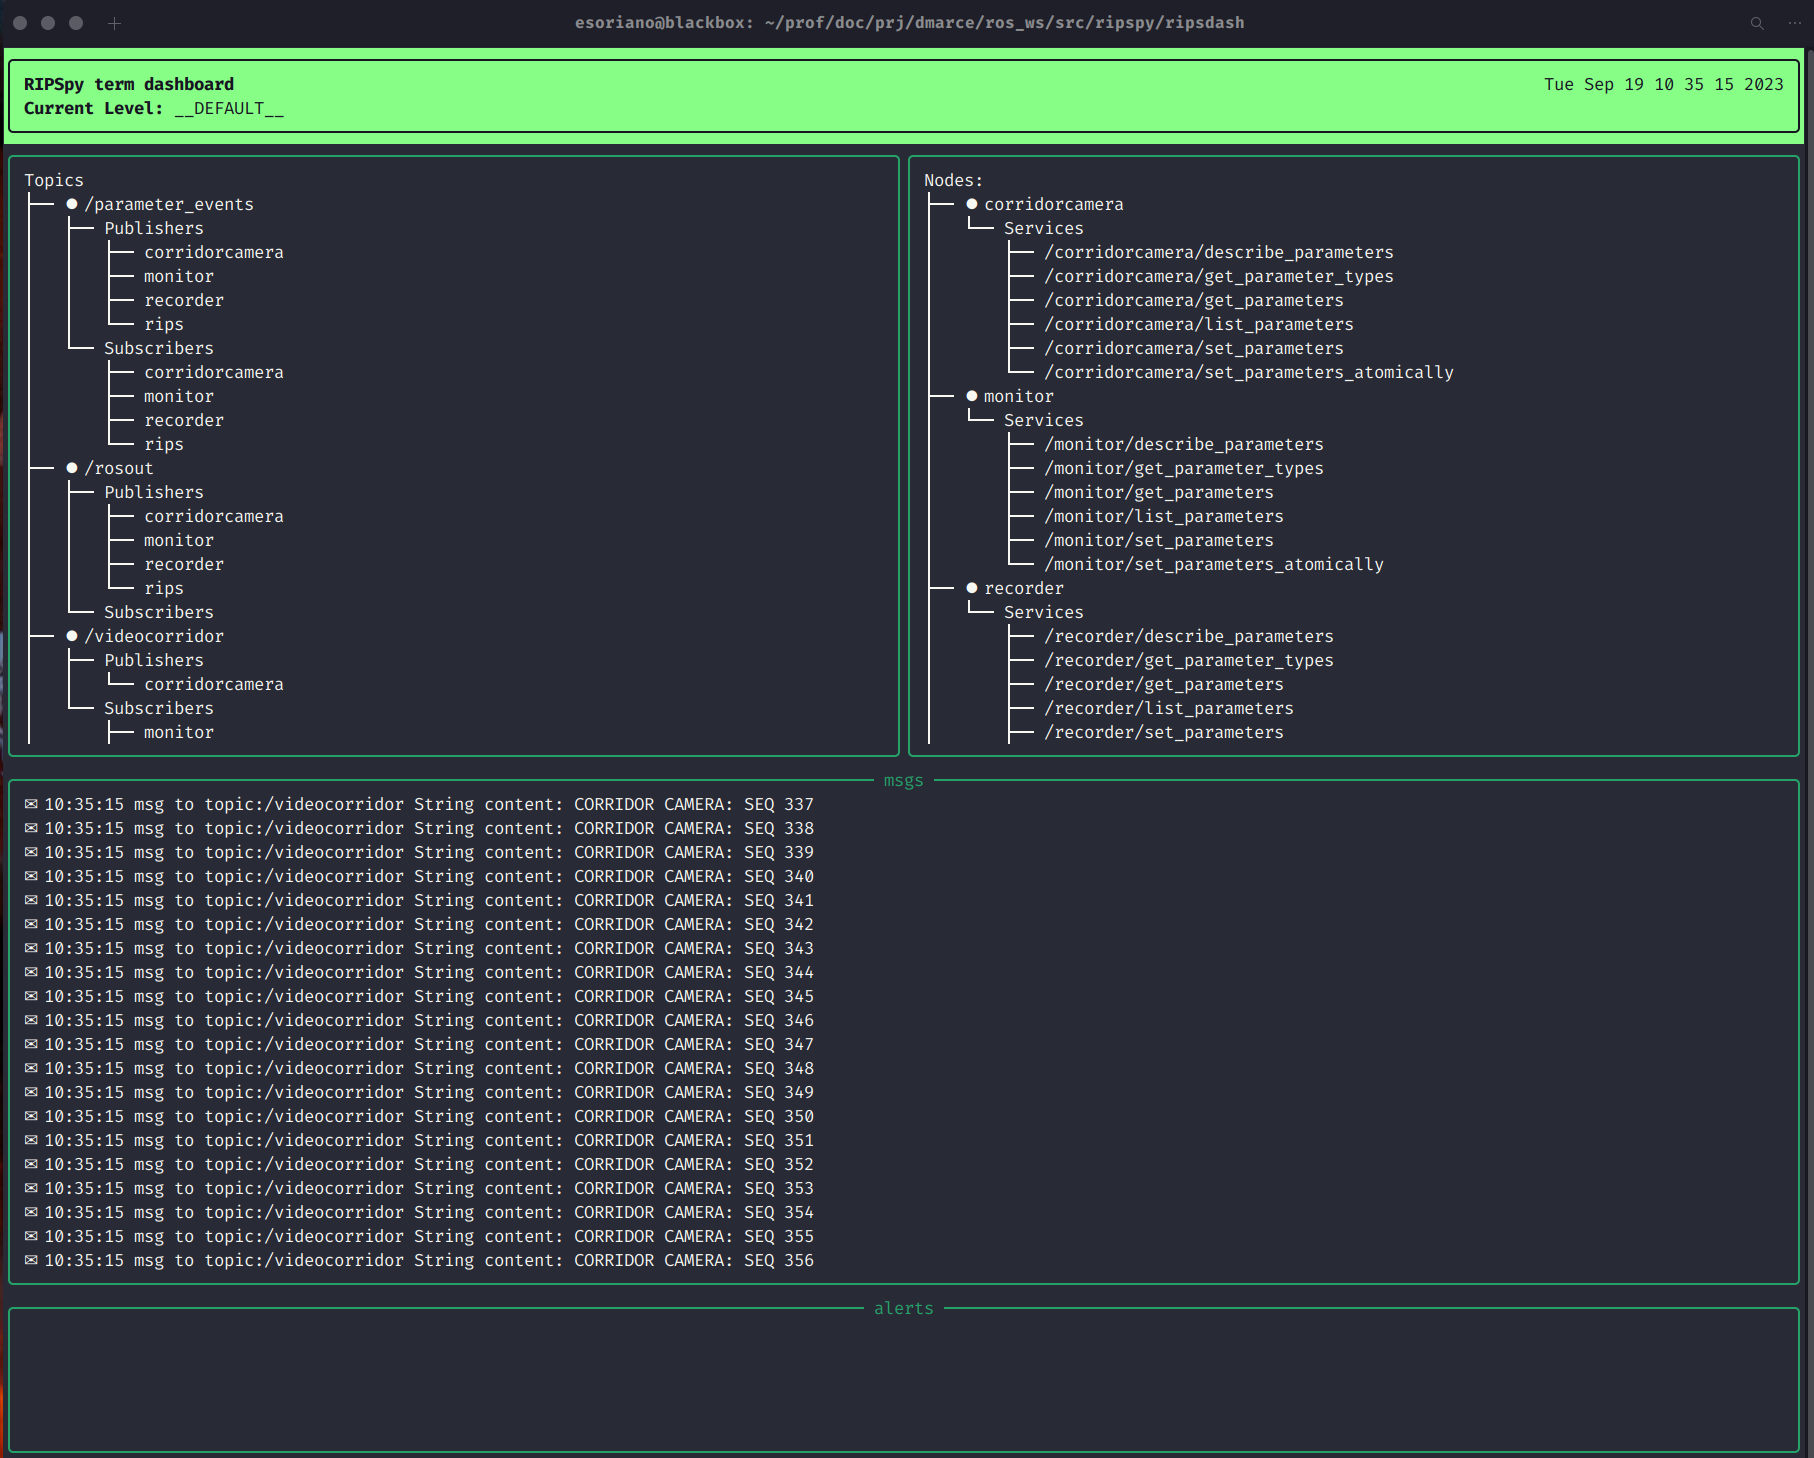
\includegraphics[width=\textwidth]{figs/ripsdash.png}
\caption{ripsdash.py executing in a Linux terminal \label{fig:dash}}
\end{center}
\end{figure}

\section{Engine: Rips \label{sect:rips}}

The program has two alternative modes of operation. As an interpreter,
it interprets a program with the rules as new messages arrive.
As a transpiler, it generates a program with the same behaviour as
the interpreter running the original program, but the generated program
can be compiled and run natively.

We have implemented the RIPS interpreter/transpiler and the code it generates
in Go~\cite{go}, for several reasons.  ROS~2~\cite{ros2} (the system in
which the RIPS runs) natively supports C++ and Python which would be the
first choices. It is desirable to use a statically typed language for
a program this complex, so we discarded Python. We could have written
the interpreter/transpiler in C++, but one of the requisites is for
it to be easy to generate a statically linked self contained program
which we can easily cross-compile for different robotic arquitectures
to test the research prototype. In this space, Go excels. We are also
very comfortable writing compilers an interpreters in Go,
as we have written various of different levels of complexity in the past.


We have programmed the interpreter/transpiler with the minimum external
dependencies and additional tools as possible, so it is easy to rewrite
in any language should the need arise later.  Linking together a Go
and Python or C++ program would make things unnecessarily complex. To
work around this problem, we decided to break the RIPS in two parts,
Ripspy (the monitor) implemented in Python and integrated natively in
ROS~2 and Rips (the engine), the interpreter/transpiler implemented in
Go which also generates Go when acting as a transpiler.  As we already
explained in the sections above, Rispsy and Rips
(be it the interpreter or the generated program; we will use the name
interchangeably) run in separate processes communicated through an IPC
mechanism (a Unix domain socket or UDS). Both together form the RIPS.
Ripspy will subscribe to the different topics, gather together the graph
state and pass messages encoded in YAML through the socket to Rips, the
Go program. The communication is bidirectional and the Rips may answer
with some YAML encoded messages of its own.


\subsection{Program example and syntax}
A simple example of a program for the Rips could be\footnote{We will provide
more examples in Appendix
\ref{sec:examples}.}:

\lstinputlisting[language=Rips]{src/example.rul}

The program could be interpreted:


\verb+./rips/rips -s /tmp/sock.777 $RIPSCONFIG/scripts $RIPSCONFIG/example.rul +

if the scripts and the socket are in its default locations, we can use the hash bang
invocation:

\verb+$RIPSCONFIG/example.rul+

it could be also transpiled:


\verb+./rips/rips $RIPSCONFIG/example.rul -c $RIPSCONFIG/scripts > gen/gen.go+


The program \texttt{gen.go} compiles to a command \texttt{gen} which would
be run like:


 \verb+./gen/gen -s /tmp/sock.777  $RIPSCONFIG/scripts+

or, if everything is in its default location:

 \verb+./gen/gen+


Both \texttt{rips} and \texttt{gen} listen to a unix domain socket in the
path they receive as parameter (\texttt{/tmp/sock.777} in the example)
and read YAML messages from it. Later they respond through the same
socket. The responses also consist on YAML messages which report level
changes and alerts.


Both programs admit the parameter \verb+-r rootpath+. It
represents the root directory from which they operate.
The programs \verb+chdir+ to the directory early, so any
relative path present in the rules or in the parameters coming
after the \verb+-r+ will be interpreted with respect to that
directory.

\subsubsection{Program Syntax}

Comments start with \# and end at the end of line.  The program is divided
into sections (\texttt{levels}, \texttt{consts}\ldots).  The section
marker is a keyword followed by a colon, with the exception of the rules
sections which have an extra keyword with the type of section.  Other than
the section marker, all the sentences end with a semicolon. Spaces and
newlines are ignored by the parser and only used to separate tokens.


\subsubsection{Levels}
A section marked \texttt{levels} enumerates the possible \emph{Alert Levels}.
Each alert level name declared in this section serves
two roles. It can be passed to a
\texttt{trigger} action to change the current state. As such, it is one of the
possible states and may have extra restrictions (like \texttt{soft})
which limit the legal transitions of the state machine. It also acts
as an integer enumerated value in expressions\footnote{To get a
string with the name see the builtin expression \texttt{levelname}
described in \ref{sec:predef}.}.  The order in which the alert levels
are declared state their alert level. Levels declared later in the
program are higher.  Rips checks which levels are reachable. A level
is reachable if there is an \texttt{trigger} action with the level as a
parameter. This error can be disabled even if the level is not reachable
by any action. For example, the rule \verb+false?trigger(UNREACHABLE_LEVEL);+ which will
never execute\footnote{It will also be deleted by the optimization phase
of the compiler.} but stops Rips from complaining about the level being unreachable.
This is an escape hatch and is present in the language on purpose.
The reachable levels are marked by the compiler before deleting dead code
instead of after, which would make the previous action not produce the
desired effect.
An \verb+int+ variable can contain a level (and be used in  \texttt{trigger},  \texttt{levelname}\ldots).
The variable has to be initialized with a level. If the variable gets out of range of the
possible levels, \texttt{trigger} will not change level and \texttt{levelname} will return a zero length string.

\subsubsection{Literals\label{sec:literals}}

Literals are a form of unnamed constants. They have a concrete type which is
\verb+(int, Universal)+, \verb+(bool, Universal)+, \verb+(string, Universal)+, or
\verb+(float, Universal)+, see~\ref{sec:types} for more details. For now, it suffices to know
that they behave as \verb+int+, \verb+bool+, \verb+int+ and \verb+float+  in any other
strictly typed programming language.

The literals for bool are \verb+true+ and \verb+false+.

Integer literals can be written in octal,
binary, or hexadecimal by preceding them with a zero followed by 'o', 'b',
'x', like in \verb+0b11101+ as well as in decimal without any prefix.
Examples are \verb+0xffe+ in hex,
\verb+0o773+ in octal, \verb+0b1101+ in binary, and \verb+12+ in decimal.

Floating point numbers need to either contain a dot or be in engineering notation
or both, like \verb+.01+, \verb+1E9+, \verb+1.02e-3+, or \verb+1e3+.

String literals are delimited by double quotes, are UTF-8 encoded and can
contain the standard escape characters. Examples are \verb+"\thello\n"+ and
\verb+"double quotes are \" and a slash is \\"+. The explicit escaped UTF-8 bytes like in
\verb+"\xe2\x86\x92"+ or the unicode code point like in \verb+"\u2192"+, both
represent a string with the code point corresponding to the right looking
arrow which could be written simply as \verb+"→"+. A string may contain
a newline, which will be interpreted literally. For example:
\begin{verbatim}
"this is a
multiline string"
\end{verbatim}
is the same as \verb+"this is a\nmultiline string"+.
If a very long string needs to be broken in multiple lines but without
newlines in the string, it can be broken with the concatenation operator
(it will still be a single literal after the constant folding pass):
\begin{verbatim}
"this is a"+
"single line string"
\end{verbatim}

\subsubsection{Consts}
A section marked \texttt{consts} is used to declare named typed constants.
The available types are the same as for literals.
They have to be initialized with a constant expression. Their lexical scope
starts  at their declaration and ends at the end of the file.

\subsubsection{Vars}
A section marked \texttt{vars} is used to declare typed global variables.
Like with constants, the available types are \texttt{string},
\texttt{int}, \texttt{bool} and \texttt{float}\footnote{All of them will be \texttt{Universal}, like
for literals.}.  They have to be
initialized with a constant expression. Their lexical scope starts  at
their declaration and ends at the end of the file.  The lifetime of these
variables will coincide with the execution of the program.  Rips will
complain if a variable is unused, unset or never accessed. Again, an
unreachable action can disable this kind of errors. For example,
 \verb+false?set(unsetvar, true);+ disables a
``\texttt{variable never set, should be a constant}" error.


\subsubsection{Rules}
A section marked \texttt{rules} will contain rules to be evaluated when
a message of the type described by the rule section type (\texttt{Graph} or
\texttt{Msg}) is received through the pipe. Another section type,
\texttt{External}, will execute with external events (signals and alerts by
the IDS of the system).

The section type (types in the language
are tuples of the type of expression and the type of the message as will
be explained later) will be
used for type checking.  Each rule contained in a section consists of
a boolean trigger expression followed by the character '\verb+?+' and a
chain of actions linked by connector operators ('\verb+=>+', '\verb+!>+'
and '\verb+,+'). Alternatively, the Unicode characters
$\rightarrow$ and $\nrightarrow$ can be used
for the arrows\footnote{They are the characters U+2192 and U+219B, which are
encoded in UTF-8 as as 0xe2, 0x86, 0x92  and  0xe2, 0x86, 0x9b respectively.}

The trigger expression is evaluated upon the arrival of
a message of the same type as the section. If the result is true, then the
actions are evaluated one by one. Depending on the result of the action
(which is a boolean value) and the connector operator, the next element
of the chain continues to be evaluated until it ends or the connector
dictates it ends.  The connector  '\verb+=>+' means \emph{``evaluate the
next action if the result of the previous action was true"}, '\verb+!>+' means \emph{``evaluate the
next action if the result of the previous action
was false''}
and '\verb+,+' means \emph{``evaluate the next action unconditionally''}.
Of course, in order for the comma connector to evaluate the following action, the chain has
to arrive to the previous action first without stopping.

Expressions can conform the trigger expression of a
rule, and can also be used within the arguments of the actions. Values
in the RIPS interpreter are all statically and strongly typed as is described next.

ROS~2 is a complex distributed system and the RIPS is
trying to detect inconsistencies and runs in a feedback loop with
the whole system. When the Rips detects something suspicious, it communicates
it to the Ripspy which may
trigger a system wide reconfiguration because of a change in the
\emph{alert level}.  This will feed back new messages with the changes
back to the Rips. Too keep all this under control, we must be completely
sure that the program the Rips is running is completely correct. This is
why the compiler is strict, statically and strongly typed, checks statically  regular
and Yara expressions, checks for the presence of the external programs it may need
later at run time, and the reachability of the \emph{alert levels} in the state machine.
In general, it tries
to error on any mistake which may be found statically.

\subsection{Type system\label{sec:types}}
As stated before, the language of the Rips is statically and strongly typed.
Variables and constants have to be declared with their types and their initial value.
Incompatible types cannot be mixed and there is no implicit casting.

The type system of Rips serves two different purposes: to prevent incorrect
operation with values and to prevent builtins to be run in the wrong section.
For example, depending on the type of message received, some builtin
functions can be called but others cannot.

Rips defines two kind of builtins, builtin expressions, which are
functions without lateral effects and builtin actions, which are procedures.
When an expression is evaluated, the result has
a type compatible only with some sections and thus
can only be used within them. Actions are universally typed
and can be called from any section.
In other words, the type of the values returned by builtin functions will
prevent the problem described above, as the Rips will check that they
are compatible with the type
of the section they are called from.

A type consists of a tuple of two subtypes \verb+(ValueType, ExprType)+,
one which is the value type (which can be \texttt{string}, \texttt{int}, \texttt{bool}
or \texttt{float}) and the other is an expression type, derived from the
type of message. The available types are \texttt{Msg}, \texttt{Graph},
\texttt{GraphMsg} and \texttt{External}.  The \emph{\texttt{Msg}} section is of type
\texttt{GraphMsg} (both the current graph and the current message can be
consulted, so both types are compatible). The \emph{\texttt{Graph}} section is of type \texttt{Graph}.
The \emph{\texttt{External}} section is of type \texttt{External}.


Internally integers and floats are kept as 64 bits signed values and
the strings are unicode.
Literals look like \verb+true+ or \verb+0b11101+ are described in \ref{sec:literals}.

Values of all types are immediate, not references
or pointers.  Strings can only be compared lexicographically and are
also treated as values, not pointers. They can also be concatenated with
the $+$ operator,
though they are truncated if they get too long.  The binary and unary
operators that can be used in expressions are roughly the same as in
C with the same precedence (with the exception of shifts which are not present\footnote{
Adding them is probably unwise without adding unsigned types.}).


There are some extra subtypes defined, \texttt{Universal} and
\texttt{Undefined}, which can act both as value subtypes or as expression
subtypes. They are compatible with any subtype. \texttt{Universal}
is used for general expressions like $(3 + 45) > 4$,
and \texttt{Undefined} to mark errors
when checking the type of erroneously mixed type expressions.


The type for two values is compatible if both subtypes in the tuple are compatible,
the value type and the expression type, otherwise the operation will result in a type with
one of the subtypes \texttt{Undefined}.
Expressions with simple types like \verb-3 + 4- have a concrete value
type and universal expression type;
\verb+(int, Universal)+ for the previous example.
Builtin functions may only be applicable to some types of messages and thus
cannot be used in any section, only in sections of a compatible type.
Their expression type is propagated to the expression containing them.

While \verb+(bool, Universal)+ is the type of a boolean expression
like \verb+true+ and \verb+(int, Msg)+ is the type of a value which uses
a message builtin expression, which can only be called within an \texttt{Msg}
compatible section and which is also compatible with an \verb+int+ expression,
of type  \verb+(int, Universal)+.

Action builtin return values are themselves universal in the expression type
(and boolean in the value), but their expression type may change depending
on their parameters.
For example the builtin call
\verb+set(isturtle, msgtypein("turtlesim"))+
has type \verb+(bool, Msg)+, the \verb+Msg+ type a
consequence of the call to \verb+msgtypein+ in the
parameter.

%add more about this and concurrency later
\subsubsection{Execution flow}
The program containing the rules will be interpreted or executed natively in a loop
(what we call the main loop). Each trigger will cause an iteration of the main loop.

The program will trigger its execution from four sources
(see the \verb+Dispatcher+ function in \texttt{extern/conc.go}), but not
all of them trigger an iteration of the main loop.
\begin{itemize}
\item When a
message is received, a main loop iteration will be executed with a message as context, for
\texttt{Graph} and \texttt{Msg} events.

\item  Whenever a \texttt{SIGUSR}
signal is received, it will be counted but a main loop iteration will not
be executed.
\item  Whenever the poller for files for
the IDS triggers, a variable will be set but a main loop iteration will not
be executed.
\item Periodically, a main loop iteration will be executed without a
message in its context (for rules reacting to \texttt{External} events).
\end{itemize}


\subsection{Alert levels state machine}
The \emph{alert levels} form a state machine. The builtin action \texttt{trigger}
changes the current alert level transitioning to a different state. The alert level
can only rise except for
\texttt{soft} levels which may be de-escalated. Levels declared with the \texttt{soft} attribute
can jump to a lower state but only the one immediately below.
The state machine from the above example is shown in Figure~\ref{fig:state}.

\begin{figure}[t!]
\begin{center}
	\includegraphics[width=\textwidth]{figs/gv_alert.pdf}
\caption{State machine \label{fig:state}}
\end{center}
\end{figure}

Note that in the example, the initial level is \texttt{A} and that the level \texttt{C} can
transition to \texttt{B} because it has the attribute \texttt{soft} in the definition.

\subsubsection{Level entry and exit programs}
Whenever a level is exited and whenever a new level is entered, an external program is run.
The programs are called like the name of the level being exited or entered followed
by an extension \texttt{.from} and \texttt{.to}
respectively.
For example, for a transition from \texttt{C}
to \texttt{D}, a program \textbf{C.from} is executed and a program \textbf{D.to} is executed.
When the program starts, only the program \textbf{A.to} is executed as the initial state
is entered.

Rips will search for these programs in a path it receives as an argument (or by
default in \texttt{/etc/rips/scripts}).
Rips will check that all of the programs are accessible and executable as part of the compilation
process.


\subsection{Predefined builtin functions\label{sec:predef}}

There are two kinds of predefined builtin functions: actions and expressions.
Actions are procedures with lateral effects and can only be used in the right part
of the rule, expressions can be used in the left part or as arguments to actions.
Builtin expressions can be used to interrogate about the current ROS~2  message or the current
state of the ROS~2  graph of nodes. Builtin actions are used to do something when a rule triggers
because the trigger expression evaluates to \verb+true+.

In the following lists, three dots indicate the function is variadic (there may
be zero or more arguments).
\\


The list of actions is:

\begin{tabular}{l}
\\
 Actions (return bool)\\
\hline\\
 set(var, value)\\
crash(msg string) \\
alert(msg string) \\
 exec(path string, args ... string)\\
 True(any ... Universal) \textbf{\#for debugging}\\
 False(any ... Universal)\textbf{\#for debugging}\\
trigger(level int)
\end{tabular}
\\

The expressions are:
\\

\begin{tabular}{l}
\\
 Msg, about the current message (return bool) \\
\hline
	msgsubtype(msgtype string, msgsubtype string)\\
	msgtypein(msgtypes  ... string)\\
	payload(pathruleyara string)\\
	plugin(path string)\\
	publishercount(min int, max int)\\
	publishers(pubs  ... string)\\
	publishersinclude(pubs ... string)\\
	subscribercount(min int, max int)	\\
	subscribers(subs  ... string)\\
	subscribersinclude(subs ... string)\\
	topicin(topics ... string)\\
	topicmatches(regex string)\\
\end{tabular}
\\

\begin{tabular}{l}
\\
 Graph, about the state of the graph (return bool)\\
\hline
	nodes(nodes  ... string)\\
	nodesinclude(nodes  ... string)\\
	nodecount(min int, max int)\\
	service(node string, srv string)\\
	servicecount(node string, min int, max int)\\
	services(node string, srvs ... string)\\
	servicesinclude(node string, srvs ... string)\\
	topiccount(min int, max int)\\
	topics(topics ... string)\\
	topicsinclude(topics ... string)\\
	topicpublishercount(topic string, min int, max int)\\
	topicpublishers(topic string, nodes ... string)\\
	topicpublishersinclude(topic string, nodes ... string)\\
	topicsubscribercount(topic string, min int, max int)\\
	topicsubscribers(topic string, nodes ... string)\\
	topicsubscribersinclude(topic string, nodes ... string)\\
\end{tabular}
\\

\begin{tabular}{l}
\\
 External, about external conditions (return bool)\\
\hline
	idsalert(alert string)\\
	signal(sig string)\\
\end{tabular}
\\

\begin{tabular}{ll}
\\
 Universal& return type\\
\hline
	levelname(level int) & string\\
	string(any Universal) & string\\
\end{tabular}
\\

The builtin action \texttt{crash} receives a string and crashes the interpreter/program
sending the string to everyone (the socket, standard error and wherever the
output is) if possible.

There are two extra builtin actions for debugging the program, \texttt{True} and \texttt{False}
both are variadic and receive any type and print it. They also return true or false
respectively.
The builtin expression \texttt{string} returns a string representation of any type.
There is also an extra builtin expression \texttt{levelname} which receives a level and returns
a string with the level name (the level itself acts as an constant integer).

The external expression \texttt{idsalert} searchs for a string in files whose name match a pattern
inside a directory (and its subdirectories). See the constants defined in \verb+ids.go+. If the
string is present, it evaluates to true.
The external expression \texttt{signal} evaluates to true when the correspondingly named
signal (either \texttt{"SIGUSR1"} or \texttt{"SIGUSR2"}) is received. If the signal is received
multiple times, the expression will evaluate to \texttt{true} multiple times. There is a counter of
signals received and it will be decremented each time
the expression evaluates to \texttt{true} so signals are not ``lost".

The external expression \texttt{plugin} executes an external command and passes
the raw message in bytes to its standard input. If there is no error and the status of the
process when exiting is zero, it will return \verb+true+ else it will return \verb+false+.

\subsection{Predefined variables}
Some variables are predeclared and automatically updated by the Rips.
\verb+CurrLevel+ contains the current level, and can be used with \texttt{trigger}  or
as an integer value in an expression.

\verb+Time+ contains the current time in nanoseconds since the Unix epoch.
\verb+Uptime+ contains the number of nanoseconds which have passed since
the Rips started.

These variables cannot be set (they are inmutable).

\subsection{Predefined constants}

Each rule has a constant defined of local lexical scope called \verb+CurrRule+ with
a unique name identifying that rule.

\subsection{Compilation}

If instead of a socket path, the command receives \verb+"-c"+, it generates a Go
package which can be compiled into a command. It depends on the \textbf{external}
package of Rips.
This commands executes natively the Rips instead of using an interpreter.

\subsection{Communication with Ripspy}

Communication with Ripspy happens through a Unix Domain Socket by
exchanging YAML encoded messages.
It is bidirectional, messages are read from the sockets and
alerts and level changes are sent back.

\subsection{Tour of the source code}

\begin{itemize}

\item[\textbf{abbench:}] Go benchmarks, both for the compiled version
and the interpreted version, with the help of two shell scripts: \texttt{bench.sh} and
\texttt{nc.sh}. It requires the constant \verb+HasStats+ to be set to true,
so the stats printed can be used by the benchmarks. It tries to estimate
how much time is spent decoding YAML, compiling, interpreting\ldots.

\item[\textbf{abtesting:}] This directory tests Rips by comparing the generated
version against the interpreted version. The Go test \texttt{ab\_test.go}
is just a wrapper around a script \texttt{ab\_test.sh}. The script
checks that the output of both programs for a rule file and a set of
messages is the same. The test runs the script with many different
rule files.
There is one caveat. When there
is a runtime panic, the error message which both programs output
is a little bit different because
each program reports its name, time and other details of the execution,
which are different. The script
filters the difference out before checking that the output is the same.

\item[\textbf{doc:}] Documentation directory. The directory \texttt{tech}
includes this tech report. The text file \texttt{GRAMMAR} details the
derivation of the LL1 grammar for the recursive descent parser. The
file \texttt{example.rul} contains an example of a valid program
for the parser.

\item[\textbf{extern:}] Go package containing
the implementation of the builtins (actions and expressions in
\texttt{actions.go} and \texttt{expr.go} respectively) and their
support, including the main functions for different goroutines.
This package is shared by the interpreter and the generated code.
Context in \texttt{context.go}  supports execution state and message
decoding. Methods to query the messages are in \texttt{msg.go}.
The file \texttt{conc.go} contains the main functions for the two principal
goroutines: the YAML message decoder and the central dispatcher.
The central dispatcher receives from different channels (for signals, events
in the IDS, new messages from ROS and from a timer) and does the
appropiate thing, including running the interpreter or generated main program.
Finally, the file \texttt{ids.go} implements the functions to watch logs for
alerts from an external IDS program.
The subdirectory \texttt{examples} contains files with YAML messages
for testing and simple examples of level exiting and entering programs
(inside of \texttt{examples/scripts}).


\item[\textbf{lex:}] The lexer. The subdirectory \texttt{examples} contains some
programs for testing the lexer.

\item[\textbf{parser:}] The parser. The file \texttt{desc.go} contains
the recursive descent parser.  The file \texttt{pratt.go} contains the
expression Pratt parser.

\item[\textbf{rips:}] Main for the transpiler/interpreter program.

\item[\textbf{tree:}] Manipulation of the AST, including the interpreter,
symbols and symbol tables.  The file \texttt{builtins.go} contains
the stubs for the builtins (and implementation of builtins that
are only interpreted like \texttt{set}. The file \texttt{gen.go} and
\texttt{genprog.go} contain the Go transpiler generator. The symbol tables and
the symbols are in \texttt{sym.go}. Support for predefined variables
in the interpreter and updating them is in \texttt{vars.go}. Constant
evaluation, folding and removing of dead code is in \texttt{const.go}. The
interpreter is in \texttt{interp.go}. The AST and its methods is
in \texttt{tree.go}. Evaluation of expressions in the tree is in
\texttt{eval.go}. Reachability of states (marked while type annotating)
is done in \texttt{states.go}. Type annotating and type checking is done
in \texttt{type.go}.

\item[\textbf{types:}] Implementation of the types, data types for them
and methods to check for type compatibility.

\item[\textbf{xrips:}] Wrapper used by the \texttt{rips} command (as an
interpreter) to enable integration and regression testing for the compiler.
The subdirectory \texttt{examples} contains various correct and
incorrect program files for testing (incorrect ones have a name matching
\texttt{$*$err.rul}). The file \texttt{errouts/okout.out} contains various
error outputs of the compiler for regression tests. A test will fail if
the errors change format, should be looked at by a human and if it is
valid, the file can be deleted and the tests ran again.

\item[\textbf{INSTALL:}] File describing how to install, compile, and test Rips.
\end{itemize}

\subsection{Transpiler implementation}
The transpiler generates a Go command in one file. It depends only on the
\texttt{extern} package and its transitive dependencies: \texttt{go-yara} and
\texttt{fsnotify} and \texttt{yaml}. The \texttt{external} package is shared with
the interpreter.

The transpiler prints parts of the program and only generates the function
in the variable \verb+runproc+.  All the code outside of that function comes
from constant strings in \texttt{genprog.go}. The function \verb+runproc+,
which will be run every single iteration of the main loop
is generated from the AST by printing it with the format
\verb+%g+ in \texttt{gen.go}. All the code generated for the
main loop iteration body  is inside that
one function and some care has been taken to make it is as simple
as possible for the Go compiler to optimize while keeping the transpiler
itself simple.  As a consequence, the generated code uses \verb+goto+ to skip over the
rules when the do not apply and it is not very human readable, though
not impossible to understand.


All the user chosen identifiers which may end up in the final program,
have a prefix prepended (a form of name mangling or name decoration)
in order not to clash with any variables defined
by the generated program.  This happens to the names of the user declared
variables and of the constants for the levels.

For example, a variable called \verb+nmsg+ in the \texttt{.rul} file
is called \verb+rul_rips_user_var_nmsg+ in the generated program.
Similarly the constant declared in the generated program for the
name of a level called \verb+HALT+ will be
\verb+rul_rips_user_level_HALT+ (the
name of the level itself will remain unchanged, the translation made via
an array of strings).

\subsection{Overview of the implementation}

\subsubsection{Lexer}
The interpreter is implemented with a simple state machine lexer coded by
hand. There was an initial version
written with continuations and trampolines and
a function for each state in the state machine. While
it was arguably cleaner, we rewrote it as a switch-case state machine
to make it simpler to understand
and easier to rewrite in any other programming language.

Token types are represented by a rune, which, when possible, is the
rune representing the lone token of the lexema (for example \verb+'*'+
for the multiplication operator). When that is not possible, for multicharacter
tokens like \verb+'>='+ or multivalued ones, like a string literal, they are
represented by values for runes which are illegal in Unicode, that is,
values which cannot represent any code point.  A type \verb+UTokType+
is used for printing error messages for the user. It is used simply to
envelope a \verb+TokType+ and make it \verb+Stringer+. \verb+TokType+
is \verb+Stringer+ but in a format more amenable to debugging.

The lexer is completely independent and decoupled from the parser and
the symbol table, i.e.  there is no \emph{lexer hack}~\cite{lexhack}.

\subsubsection{Parser}
The parser is implemented as a recursive descent parser with a Pratt
subparser~\cite{pratt} for expressions.  The reason for this separation
is that an \emph{LL1} grammar expressing so many levels of precedence
gets unbearably complex.


Similar to the original Pratt parser described in~\cite{pratt}, it is built from
three methods, \verb+Expr+, \verb+Nud+ and \verb+Led+.  The method
\verb+Nud+ parses a naked subexpression without context.  The method
\verb+Led+ parses a subexpression with a left context. This happens
when the subexpression to the right is composed of a higher precedence
operator than the one on the right. The left subexpression is kept as the
left context argument to \verb+Led+ and the tree is glued together later.
The method \verb+Expr+ iterates
through an expression, calling \verb+Nud+ and \verb+Led+ as needed
depending on the binding power of the operators.  The three are mutually
recursive. \verb+Nud+ represents a single term and only calls \verb+Expr+ when
it processes a parenthesized expression.
This is similar to the Shunting-yard Algorithm~\cite{dijkstra1961algol}
or the Precedence Climbing algorithm~\cite{richards1981bcpl} but using
the stack of the compiler instead of a separate data structure.


The Pratt parser is not like the original Pratt parser, which used a
function for each \emph{nud} and \emph{led} type but table driven. There are
tables for the binding power of each kind of token and stating if they
are unary, binary and so on.
This makes the parser considerably shorter and more understandable
when written in Go.

Go has unlimited stacks (originally segmented, in later versions reallocated),
making it perfect for any kind of recursive implementation,
as there are no arbitrary size limits to the stack size.

\subsubsection{AST}
We implemented the AST with a symbol type record, \verb+Sym+, which we use
whenever more than one type can hang from the tree. For example
in an expression one term can be an integer value or a subexpression.
This is generally called the \emph{expression problem}~\cite{exprprob}.
The \verb+Sym+ type record represents the union of all these kind of elements by
having a symbol type identifier field, \verb+SType+ containing different pointers to the
the subtypes and values for each scalar subtype. The ones which are not
relevant for the current type should be ignored and will contain the zero value.
Go does not have tagged types
or algebraic data types which are both a different way of solving this problem,
but there is another alternative to the approach we have taken.
We could have used tagged interfaces, that is, \verb+Sym+ could be an interface
with an empty method \verb+IsSym+ which all the symbol types
(expression, float value and so on) implement and we hang a \verb+Sym+ interface
from the tree.

Later types switches can be used to recover the original type.
This makes the code much longer and somewhat more difficult to
read because of the bureaucracy of wrangling with the types
as they go in and out of the functions and methods.
One of the benefits of algebraic types is not present in Go, the switches being
exhaustive and alerting the programmer if some
types where left out.
Both ways of programming the AST, tagged interfaces or doing the switch by hand,
have things for and against them.
We finally took the one which we were sure we could rewrite easily in any
programming language in case this is needed later. We explicitly put the
information in the \verb+Sym+ record with a type field containing an enumerated
value expressing which fields
are to be taken in account depending on what the record represents.

The AST itself hangs from the record of type \verb+Prog+.
There is a symbol table for scoping, a stack of maps from strings to \verb+Sym+ pointers
called \verb+StkEnv+.

A type \verb+USym+ is defined to print error messages for the
user. It is used simply to envelope a \verb+Sym+ pointer and make it
\verb+Stringer+. The type \verb+Sym+ pointer is \verb+Stringer+ but in a format more
amenable to debugging. There are two format verbs, \verb+%s+ to print
the symbol themselves and \verb+%t+ to print their type.

\subsubsection{Evaluation}

The function to evaluate a tree representing an expression is the
\verb+Sym+ method \verb+EvalExpr+. This function is used at compilation
time to evaluate constant expressions and called from the interpreter at
runtime. In both cases it is called with an environment stack containing the
current identifiers in scope. At runtime it represents the execution
environment, at compilation time, the lexical environment.  At runtime, an
extra execution context is passed (at compile time it is set to \verb+nil+),
which contains details of the current message, the different existing alert levels, etc.

\subsubsection{Passes on the AST}
After building the AST, there are four passes.  The first one
annotates types. The tree is annotated with the type synthesized from the leaves.
Type errors are annotated in the expression part of the type as
\texttt{Undefined}.  The second pass does the actual type checking and
reporting of errors.
The third one does constant folding, dead code elimination and
compilation of external subprograms (Yara rules and regular expressions).
The fourth and final passes check levels: programs for entry and exit and reachability,
which was also marked in the annotation pass.

The third pass guarantees that Yara and regular expressions are correct before
starting the message processing. A builtin like \texttt{topicmatches},
which receives as argument a string with a regular expression and will have
its argument switched with a precompiled regular expression in this phase.

Later when the builtin implementation is called, the expression is
already precompiled and the matching is faster.
The same happens with the Yara rules, which are compiled and interpreted
by a pure self-contained Go Yara implementation~\cite{goyara}.  This is
not done for the transpiled program, which will compile expressions on
first use and cache the result, but the compiler has already checked
the expressions for correctness, so they are guaranteed to compile at
runtime as long as the Yara rule files are not modified.
At runtime, the program listens on a
socket for YAML encoded ROS~2 messages, and triggers the rules as needed.

\subsubsection{Errors and error recovery}

Error management, report and recovery is one of the most difficult
subjects when writing a parser or a program in general. In this sections
we explain the different strategies we have wielded to keep the complexity
at bay while giving good error messages to the user.


\subsubsection{Error management in the lexer}

The lexer is a simple state machine. It is called by the lexer. In turn,
it calls Go buffered input output.
We wrapped Go \verb+bufio+ with three private methods from the lexer \verb+get+, \verb+unget+ and
\verb+accept+. They read a rune or return it while keeping past read runes in
an array. Accept returns the array and empties it. They keep account of the number of lines read
to add to error reporting later. The state machine is quite simple
code, runes are peeked (by getting them and returning them if they are not the right ones)
and if they correspond to the prefix of a token, the state machine advances. Two kind of errors may
happen in the lexer. Errors from the underlying read (we do not consider reaching the end
of file an error, it is messaged with a special rune) or errors because a token is invalid.
It does not make sense to control for errors each time a \verb+get+ or \verb+unget+ is performed,
as all errors of this kind will be forwared to the \verb+Lex+ function to return an error. We use
\verb+panic+ for this.
The two methods \verb+get+ and \verb+unget+ panic and are recovered at the highest
level by \verb+Lex+ which returns an error. All the other errors of the lexing itself are
reported by returning error values when needed. The same recover will
deal with any runtime panic inside the lexer and continue as normal.

\subsubsection{Error management and recovery in the parser}

There is also a \verb+recover+ at the top of the \verb+Parse+ method, but it is for dealing with runtime
panics only. Another \verb+recover+ exists at the top of
the \verb+EvalExpr+ symbol method to account for bad
arithmetic operations like \emph{division by zero}. They recover the panic and return
a regular error.
There is another deferred function call at the top of the Pratt parser, in the \verb+Expr+ function,
just to make sure that if the expression returned is \verb+nil+, an error value is returned.
This is probably unneeded, just defensive programming in case of a mistake.

The main strategy for dealing with parsing errors in the parser is calling the method
\verb+Errorf+, then  trying to resynchronize and recover if needed and finally continue parsing.
The method \verb+Errorf+ reports the error to the user and counts the number
of errors. If there are too many, it panics,
which will be recovered by the parse function, delete the program and prepare everything for
exiting.

Whenever there is a parsing error, the parser needs to recover. What it does depends on the kind of
error. If it knows what token was expected,
it may be possible to insert it (i.e. continue as if there was no error).
Else, it needs to resynchronize.
In most cases, the method \verb+matchErr+ tries to find a known token and if it is not found,
it reports the problem to the user and resynchronizes using \verb+NextSync+ to find a synchronizing token.
In some other cases, \verb+NextSync+ or one of its variants is called directly after an error.
For example, some times at the end of a sentence which has the semicolon in the calling function,
\verb+NextSyncNoSemi+ is called to make sure that the compiler can proceed normally after returning.
Another interesting case happens when there is an empty clause in the grammar and an error
happens. In that case, if we are at the end of a section, checked by \verb+IsEndSection+, we make
sure there is no recurring call, so that the parser continues progressing.

% match, matchErr
% NextSync
% NextSyncNoSemi
% NextSection

\appendix

\section{Example Rule Files \label{sec:examples}}

In the following examples, we use the voice synthesis command \texttt{spd-say} to
warn the user.

\subsection{Example 1}

If the number of nodes is greater than the maximum (defined by the
constant \texttt{MaxNodes}), the engine changes the current level to
\texttt{ALERT}.  If the number of nodes decreases and is less than
the maximum, the level is set to \texttt{\_\_DEFAULT\_\_} again (because
\texttt{ALERT} is \textit{soft}).

When the number of subscribers and publishers
for the topics \texttt{/videocorridor} and \texttt{/videoffice}
is out of range, the level is changed to \texttt{COMPROMISED}.

Only the node \texttt{corridorcamera} should publish in the
topic \texttt{/videocorridor}. If any other node publishes in this topic,
the system changes the current level to \texttt{HALT}.

\lstinputlisting[language=Rips]{src/r1.rul}

\subsection{Example 2}

The \texttt{Graph} rules are similar to the ones in the previous example.
This file was used to test the signal handling. When the Unix signal
\texttt{USR1} is sent to the \texttt{rips} process, the system changes
the current level to \texttt{HALT}.

\lstinputlisting[language=Rips]{src/r2.rul}


\subsection{Example 3}

This example shows a rule using the YARA function. YARA is widely
used to detect malicious payloads, today it is the \textit{de facto}
standard for describing binary patrons and malware signatures.

The engine will invoke \texttt{yara} for each received message. If any of the
patterns defined by the YARA rules of the file\texttt{/var/tmp/yara.yar}
are found in the raw payload of the message,
the system warns the user and
changes the current level to \texttt{HALT}.

\lstinputlisting[language=Rips]{src/r3.rul}

\subsection{Example 4}

This example test the functions that inspect the types of the messages
and the variables of our language. For each received message, two boolean
variables are used to detect if its type is \texttt{ParameterEvent} or
\texttt{String}. In this case,
the system sends an alert,
changes the current level to the \texttt{COMPROMISED} level and
increments the counter. Then, the two variables are reset.
When the counter reaches a maximum value (defined by the constant
\texttt{MaxBadMsgs}), the system sends an alert, warns the user and
changes the current level to \texttt{HALT}.

\lstinputlisting[language=Rips]{src/r4.rul}


\subsection{Example 5}

This example uses a RIPS plugin, which is executed for every message
received. If the plugins exits with success, the function returns
true and the rule is triggered. The actions of this rule are sending
an alert, warning the user and changing the current level to \texttt{HALT}.

\lstinputlisting[language=Rips]{src/r5.rul}

This plugin is a Python program. Note that a plugin can be implemented
in any language. The standard input of the process that executes the plugin
will be the raw message received by the engine.

In this case, this program
uses the ROS 2 libraries to inspect the fields of the received message.
It tries to de-serialize a message of type \texttt{std\_msg/msg/String}.
Then, it inspects the fields of the message. If their values match with
some values (``patata'', etc.), the program exits successfully. Else,
it exits with failure (so the RIPS rule will not be triggered).

\lstinputlisting[language=Python]{src/plugin.py}


\section{Formal grammar}
This is the LL1 grammar~\cite{aho2007compilers} of the language, excluding \texttt{EXPR}.
That sublanguage
is delegated to the Pratt~\cite{pratt} parser.
\begin{verbatim}
PROG := 'levels' ':' LEVELDECLS' PROG |
        'vars' ':' VARDECLS PROG |
        'rules' ID ':' ACTIONDECLS PROG |
         empty

CONSTDECLS := ID ID '=' EXPR ';' CONSTDECLS |
              empty

VARDECLS :=	ID ID '=' EXPR ';' VARDECLS |
            empty

LEVELDECLS := ID ATTROPT ';' LEVELDECLS |
              empty

ATTROPT := 'soft' |
            empty

ACTIONDECLS := EXPR '?' RULER ';' ACTIONDECLS |
               empty

RULER :=	EXPR ACTSEQ |

ACTSEQ := '=>' RULER |
          '!>' RULER
          ',' RULER
           empty
\end{verbatim}
The grammar for the Pratt parser is:
\begin{verbatim}
EXPR := '!' EXPR |
         '~' EXPR |
         '(' EXPR ')' |
         EXPR '+' EXPR |
         EXPR '-' EXPR |
         EXPR '/' EXPR |
         EXPR '*' EXPR |
         EXPR '%' EXPR |
         EXPR '^' EXPR |
         EXPR '||' EXPR |
         EXPR '&&' EXPR |
         EXPR '>' EXPR |
         EXPR '>=' EXPR |
         EXPR '<' EXPR |
         EXPR '<=' EXPR |
         EXPR '|' EXPR |
         EXPR '&' EXPR |
\end{verbatim}
The semantics and precedence for expression operators is similar
to that of C. All binary operators are left associative.
\bibliographystyle{ieeetr}
\bibliography{tech}
\end{document}
